\documentclass[colorlinks,aspectratio=169]{beamer}

\usepackage{graphicx}
\usepackage[spanish]{babel}
\usepackage[utf8]{inputenc}

\usefonttheme{professionalfonts}
\usetheme{Madrid}
% Bergen, Boadilla, Copenhagen, Dresden, Hannover, Luebeck, AnnArbor, Berkeley, Darmstadt, Frankfurt, Ilmenau, Madrid, Warsaw, Antibes, Berlin, CambridgeUS, Malmoe, PaloAlto
%\setBeamercovered{transparent}

\begin{document}

\title{Ejemplo de una presentación usando Beamer}
\author[iniciales de autor(a)]{Autor(a)} 
\date{\today}
\frame{\titlepage}

\begin{frame}
\frametitle{Contenidos}
\tableofcontents
\end{frame}

\section{Introducción}
\begin{frame}\frametitle{Título de la lámina}
Contenido de la lámina
\end{frame}

\begin{frame}\frametitle{Ejemplo con un bloque}
Podemos incluir un ``bloque'', usando el entorno \texttt{block}
\begin{block}{Nombre del bloque}
Una ecuación dentro del bloque
\begin{equation}
\nabla^2\Psi=0
\end{equation}
\end{block}
\end{frame}

\begin{frame}
\frametitle{Ejemplos de figuras}
Puedes incluir figuras de manera fácil y con opciones de personalización. Por ejemplo, esta figura:
\begin{figure}[ht]
\centering
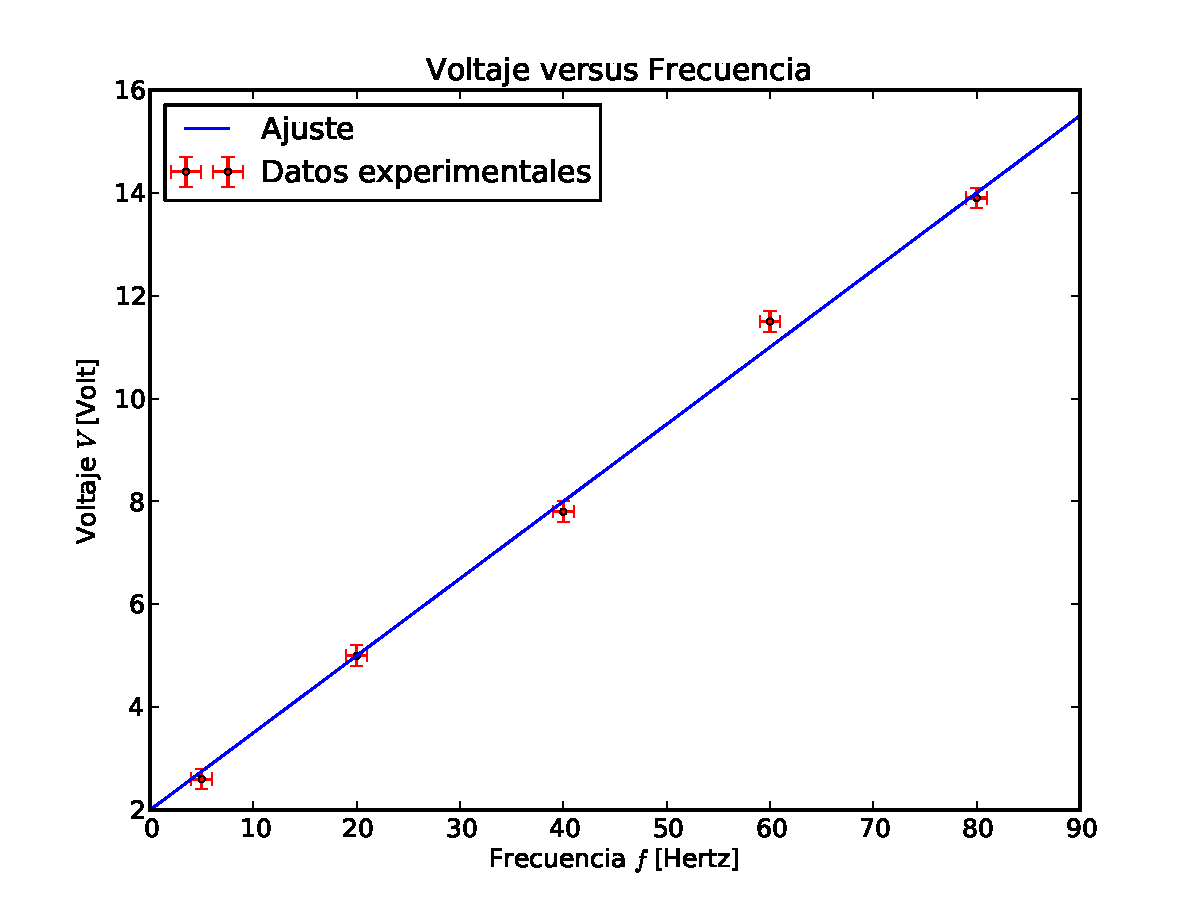
\includegraphics[width=0.4\textwidth]{fig-ajuste-lineal.pdf}
\caption{Ejemplo de figura}
\label{fig:ejemplo}
\end{figure}
\end{frame}

\section{Conclusión}

\begin{frame}
\frametitle{Conclusión}
\begin{alertblock}{En resumen}
Contenido de un bloque de alerta
\end{alertblock}

\begin{exampleblock}{En resumen}
Contenido de un bloque de ejemplo
\end{exampleblock}
\end{frame}
\end{document}
